\documentclass[a4paper,14pt]{article}

\usepackage{comment} % Para comentar várias linhas ao mesmo tempo

%matemática
\usepackage{amsmath}
\usepackage{amssymb}

%diagramação
\usepackage{extsizes}
\everymath{\displaystyle}
\usepackage{geometry}
\usepackage{fancyhdr}
\usepackage{multicol}
\usepackage{graphicx}
\usepackage[brazil]{babel}
\usepackage[shortlabels]{enumitem}
\usepackage{cancel}
\usepackage{textcomp}
\usepackage{tcolorbox}

%tabelas
\usepackage{array} % Para melhor formatação de tabelas
\usepackage{longtable}
\usepackage{booktabs}  % Para linhas horizontais mais bonitas
\usepackage{float}   % Para usar o modificador [H]
\usepackage{caption} % Para usar legendas em tabelas
\usepackage{wrapfig} % Para usar tabelas e figuras flutuantes


%tikzpicture
\usepackage{tikz}
\usepackage{scalerel}
\usepackage{pict2e}
\usepackage{tkz-euclide}
\usetikzlibrary{calc}
\usetikzlibrary{patterns,arrows.meta}
\usetikzlibrary{shadows}
\usetikzlibrary{external}

%pgfplots
\usepackage{pgfplots}
\pgfplotsset{compat=newest}
\usepgfplotslibrary{statistics}
\usepgfplotslibrary{fillbetween}

%colours
\usepackage{xcolor}



\columnsep=2cm
\hoffset=0cm
\textwidth=8cm
\setlength{\columnseprule}{.1pt}
\setlength{\columnsep}{2cm}
\renewcommand{\headrulewidth}{0pt}
\geometry{top=1in, bottom=1in, left=0.7in, right=0.5in}

\pagestyle{fancy}
\fancyhf{}
\fancyfoot[C]{\thepage}

\begin{document}
	
	\noindent\textbf{6FMA06 - Matemática} 
	
	\begin{center}Descrevendo situações com formas descritivas (Versão estudante)
	\end{center}
	
	\noindent\textbf{Nome:} \underline{\hspace{10cm}}
	\noindent\textbf{Data:} \underline{\hspace{4cm}}
	
	%\section*{Questões de Matemática}
	
	\begin{multicols}{2}
		\noindent Formas descritivas são usadas para descrever situações. Os exercícios desta aula nos fornecem alguns exemplos. \\
		\noindent\textsubscript{-----------------------------------------------------------------------}
		\begin{enumerate}
			\item A soma de dois números é 10. Se um número é 3, escreva uma forma descritiva do outro número. \\\\\\\\\\\\
			\item A soma de dois números é $k$. Se um número é $n$, escreva uma forma descritiva do outro número. \\\\\\\\\\\\
			\item O produto de dois números é $p$. Se $q$ é um dos números, escreva uma forma descritiva do outro número. \\\\\\\\\\
			\item Você está no andar $a$ de um edifício e desce $d$ andares. Escreva uma forma descritiva do andar em que você chegará. \\\\\\\\\\\\\\\\\\\\
			\item Descreva a área do retângulo abaixo de mais de uma maneira. Explique os diferentes sentidos.
			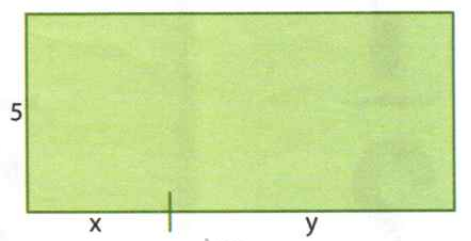
\includegraphics[width=1\linewidth]{6FMA06_imagens/imagem1}
			\newpage
			\item Um retângulo tem os lados tais que um deles é o dobro do outro. Escreva uma forma descritiva da área desse retângulo. \\\\\\\\\\\\\\\\\\\\\\\\\\\\
			\item Um estudante dispõe de três camisetas (uma verde, uma azul e uma amarela) e duas bermudas (uma branca e uma preta). Escreva uma forma descritiva do número de modos distintos que ele pode se vestir. \\\\\\\\\\\\\\\\\\\\\\\\\\\\\\\\
			\textbf{Desafio olímpico} \\
			\\
			Onde está a letra $A$? \\
			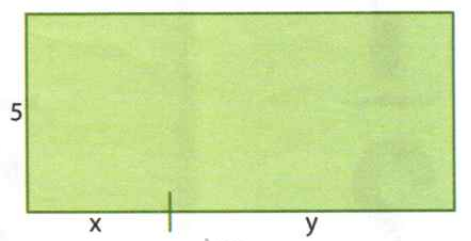
\includegraphics[width=1\linewidth]{6FMA06_imagens/imagem1}
			\begin{enumerate}[a)]
				\item Dentro do círculo e do retângulo, mas fora do triângulo.
				\item Dentro do triângulo e do retângulo, mas fora do círculo.
				\item Dentro do círculo e do triângulo, mas fora do retângulo.
				\item Dentro do retângulo, mas fora do triângulo e do círculo.
				\item Dentro do círculo, mas fora do retângulo e do triângulo.
			\end{enumerate}
			%19 a 23
			\item A soma de dois números é 29 e um deles é 12.
			\begin{enumerate}[a)]
				\item Usando subtração, escreva uma descrição do outro número. \newpage
				\item Qual é o outro número? \\\\\\\\\\\\\\\\\\
			\end{enumerate}
			\item Escreva duas descrições da área do retângulo abaixo. \\
			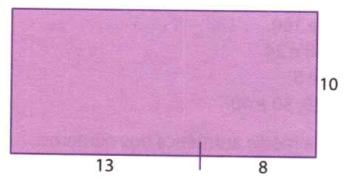
\includegraphics[width=1\linewidth]{6FMA06_imagens/imagem3}
			\\\\\\\\\\\\\\\\\\\\\\\\\\\\\\\\\\\\\\\\\\\\
			\item O número de livros de Matemática que André possui é o dobro do número de livros de Português, e o número de livros de Geografia é o quíntuplo do número de livros de Português.
			\begin{enumerate}[a)]
				\item Sendo $x$ o número de livros de Português, escreva o número de livros de Matemática, Português e Geografia que André possui. \\\\\\\\\\\\\\\\\\\\\\\\
				\item Sendo $y$ o número de livros de Matemática, escreva o número de livros de Matemática, Português e Geografia que André possui. \\\\\\\\\\\\\\\\\\\\\\\\
				\item Sendo $z$ o número de livros de Geografia, escreva o número de livros de Matemática, Português e Geografia que André possui. \\\\\\\\\\\\\\\\\\
			\end{enumerate}
			\item Uma escola tem 47 salas de aula e todas elas têm exatamente $x$ meninos e $y$ meninas. Escreva uma forma descritiva para indicar o número de alunos que assistem aula nessa escola. \\\\\\\\\\\\\\\\\\\\\\\\\\\\\\\\\\\\\\\\
			\item Um avião, que estava a 13 650 m de altura, desceu 2 437 m.
			\begin{enumerate}[a)]
				\item Escreva, usando subtração, uma descrição da nova altura em que está o avião.  \\\\\\\\\\\\\\\\\\
				\item Qual a nova altura do avião?
			\end{enumerate}
		\end{enumerate}
		$~$ \\ $~$ \\ $~$ \\ $~$ \\ $~$ \\ $~$ \\ $~$ \\ $~$ \\ $~$ \\ $~$ \\ $~$ \\ $~$ \\ $~$ \\ $~$ \\ $~$ \\ $~$ \\ $~$ \\ $~$ \\ $~$ \\ $~$ \\ $~$ \\ $~$ \\ $~$ \\ $~$ \\ $~$
	\end{multicols}
\end{document}